
\documentclass[14pt]{extarticle}
\usepackage{graphicx}
\usepackage{pdfpages}
\usepackage[T1]{fontenc}
\usepackage[margin=1in]{geometry}

\graphicspath{ {./images/} }

\begin{document}
    \pagenumbering{arabic}
    \pagestyle{plain}

    \title{\Huge Assignment 5\\ Computer Networks}
    \author{\huge Vikas Gola : 2016UCS0023}
    \maketitle
    \newpage

    \noindent
    \textbf{\large Question 1}
    Write a brief note on the meaning of each component of both the structures in\_addr and sockaddr\_in.\\[10pt]
    \textbf{\large Answer}
    \begin{itemize}
        \item \textbf{struct in\_addr:} This structure contains only one member which is s\_addr of type u\_long type
        for storing the 32 bits IP address which can be netID or hostID.
        \item \textbf{struct sockaddr\_in:} This structure contains 4 members total of 16 bytes. sin\_family that is of 2 bytes of type short and used to 
        store the family type of socket e.g. AF\_INET, AF\_UNIX. sin\_port that is also of 2 bytes of type u\_short (unsigned short) stores port number of
        host machine e.g. 23, 9939. sin\_addr is of 4 byte of type in\_addr that already has been discussed in last point which used to store the
        IP address of host machine. sin\_zero of 8 byte of type char array which may be used in future or can be used to extra info about address.
    \end{itemize}
    \vspace{1cm}


    \noindent
    \textbf{\large Question 2}
    Write  a  program  with  two  functions:  
    (1)  First  function  takes  an  IPA  as  argument  from  the  user  onthe command line 
    (i.e.  in the form of a string) and populates the structure sockaddrinwith the IPA  in  the  NBO
    using  the  function  intinetaton(const char*cp, struct inaddr*inp) 
    (2) Second, reads the IPA from an already populated structure 
    and prints the IPA in the string format using the counterpart function int inet\_ntoa(const char*cp, struct inaddr*inp)\\[10pt]
    \textbf{\large Answer}
    Both function has been implemented in program with filename q2.c
    \begin{itemize}
        \item \textbf{(1)} First function name is \textsf{void populateSockAddr(struct sockaddr\_in *addr)}.
        \item \textbf{(2)} Second function name is \textsf{void printPopulatedAddr(struct sockaddr\_in addr)}.
    \end{itemize}
    \vspace{1cm}

    \noindent
    \textbf{\large Question 3}
    As discussed in class, the Intel machines are little-endian machines whereas 
    the NBO is big-endian.  Using the logic discussed in the class, 
    write a program that detects and prints whether a machine is a little-endian or a big-endian. 
    Write another program that would - convert the same to network byte order andgiven an IPA 
    and port number in network byte order, 
    would convert the same to the host byte order.\\[10pt]
    \textbf{\large Answer}
    First and Second program is written in file with name q3.1.c and q3.2.c respectively\\
    \vspace{1cm}

    \noindent
    \textbf{\large Question 4}
    Write a tcp client program that does not use bind() function,
     but relies upon the kernel to providean IPA and port number. 
     Since the IPA and port number are provided by the kernel, 
     write a function which obtains the local socket name using the call viz. 
     int getsockname(int sockfd, structsockaddr*localaddr, socklett*addrlen) and 
     displays the allocated IPA and port numbers. 
    Look up the man pages of getsockname to learn how to use this function.\\[10pt]
    \textbf{\large Answer}
    Program is written in file with name q4.c
    \vspace{1cm}

    \noindent
    \textbf{\large Question 5}
    Write a program that takes multiple command line arguments 
    (which  are  machine  names)  and  usesappropriate function to print their IP addresses. 
    Write its counterpart that takes multiple command linearguments (which are IP addresses) and uses appropriate function to print their hostnames. 
    Include an additional option which determines which function to invoke and which argument to take.\\[10pt]
    \textbf{\large Answer}
    Program is written in file with name q5.c
    \vspace{1cm}

    \noindent
    \textbf{\large Question 6}
    Modify the TCP and UDP dautime service client illustrated in the lab to display the hostname and theport number of the server, 
    also along with the time of the day. Recollect that he daytime client uses thedatyime service running on port no 13 on the server to fetch the time of the day from the server anddisplay the same on the standard output on the client side.\\[10pt]
    \textbf{\large Answer}
    Programs of daytime service with TCP are written in files with name q6.tcpclient.c and q6.tcpserver.c\\
    and Programs of daytime service with UDP are written in files with name q6.udpclient.c and q6.udpserver.c
    \vspace{1cm}

    \noindent
    \textbf{\large Question 7}
    Now modify the client in the problem number 6 that requests an iterative TCP server on port no 99XX(XX are the last two digits of your IIT enrollement number) to send it the time of the day.
    The serverupon  receiving  the  client  request  responds  with  the  time  of  the  day,  which  the  client  outputs  on  thestandard output, along with the hostname and the port number of the server. 
    Now start thetcpdumpwith appropriate arguments (refer \$man tcpdump) to capture packets from or to a remote host.  Afteryou have started the TCP server and the TCP client terminate tcpdump, 
    examine its output and make appropriate inferences based on the output.\\[10pt]
    \textbf{\large Answer}
    Total packets captured : 8\\
    3 packets for 3 way handshake\\
    1 packet for data sending\\
    4 packets for 4 way handshake.\\[10pt]
    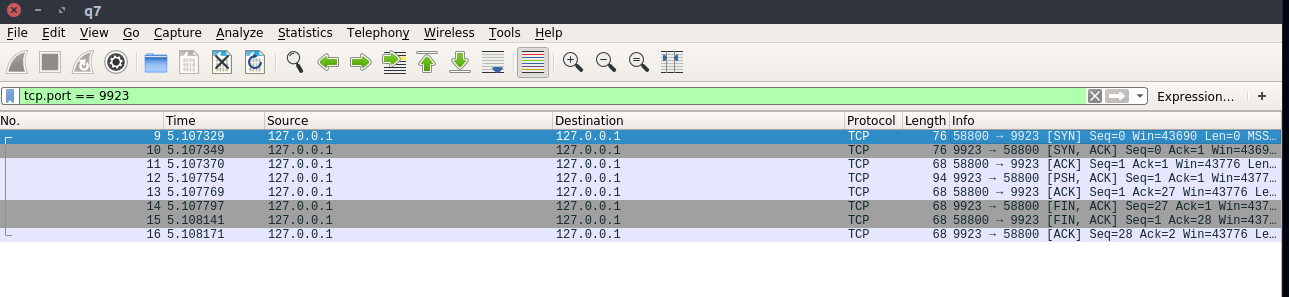
\includegraphics[scale=0.35]{images/q7.png}
    \vspace{1cm}

    \noindent
    \textbf{\large Question 8}
    Repeat the exercise in Problem no 7, but now with UDP as the underlying Transport protocol.\\[10pt]
    \textbf{\large Answer}
    Total packets captured : 2\\
    1 packet for sending message "please send me time" or known as hello message from client to server.\\
    1 packet for sending time to client from server.\\[10pt]
    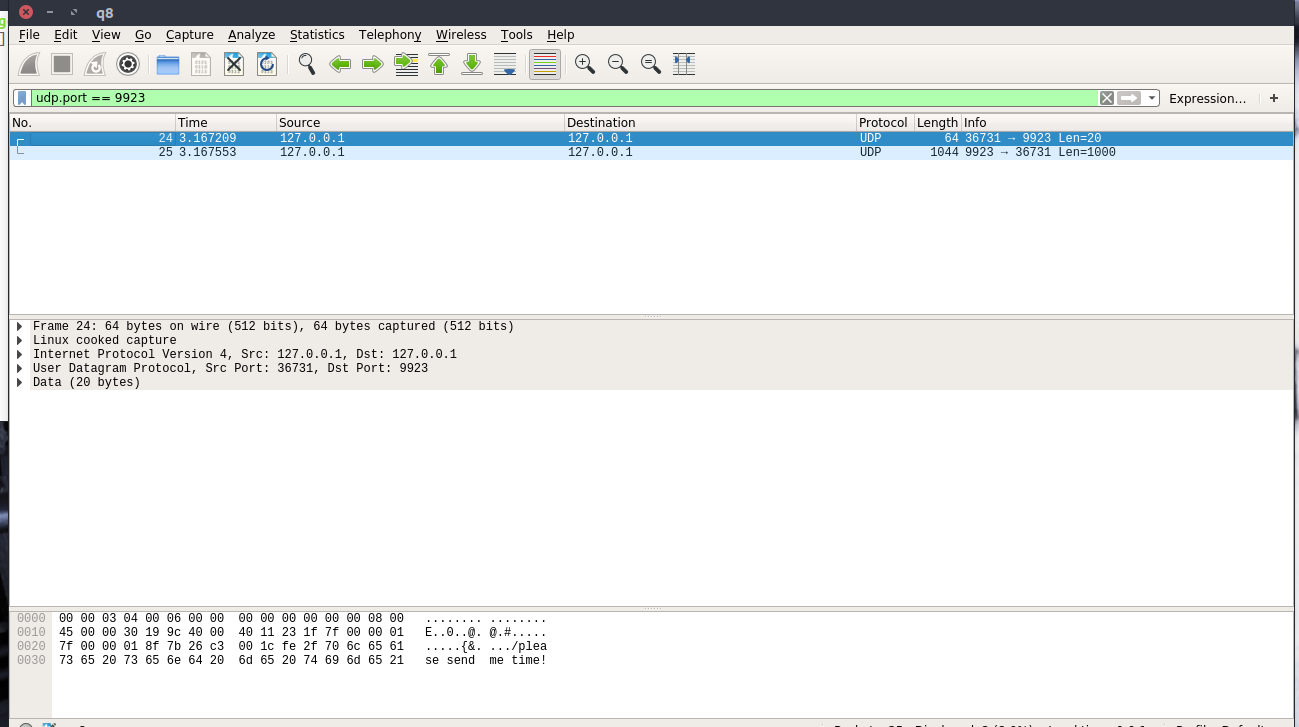
\includegraphics[scale=0.35]{images/q8.png}
    \vspace{1cm}

    \noindent
    \textbf{\large Question 9}
    Modify the server program in problem 7 to make it work as a concurrent server.2\\[10pt]
    \textbf{\large Answer}
    Program filename: q9.c
    \vspace{1cm}

\end{document}